%
% clip.tex
%
% (c) 2024 Lukas Schöpf, OST Ostschweizer Fachhochschule
%


\chapter{Cross-modal networks
    \label{chapter:crossmodalnetworks}}
    Multimodal deep learning is the study of models that learn from multiple modalities.
    For example, a human can use both vision and hearing to identify an object or a person.
    Cross-modal deep learning, on the other hand, uses data from one modality to improve performance in another.
    For example, if a human looks at a picture of a bird and listens to the bird's song, they might be able to identify the bird.
    
    Its most impressive feature is the ability to perform well on data on which the model has not been trained.
    This ability is called zero-shot capability, which is derived from N-shot capability.
    N-shot capability describes how many training samples of a particular class a model needs to classify it correctly.

    In this work, cross-modal networks are used to find relationships between images and text.
    Networks which are trained for this task are called Contrastive Language-Image Pre-training models.
    Most cross-modal networks built for this task consist of a text encoder and an image encoder.

    \section{Text encoder}
    The text encoder is in most cases a transformer (see \cref{fig:crossmodalnetworks:textencoder}).
    It encodes a given text into a high dimensional vector space.
    The closer 2 words are related, the closer their embedded vectors are to each other.
    This high dimensional vector space allows the transformer to classify unseen classes quit correctly because their vector is close to related classes.
    For example the vector for cat shoud be close to the vector for dog.

    \begin{figure}
        \centering
        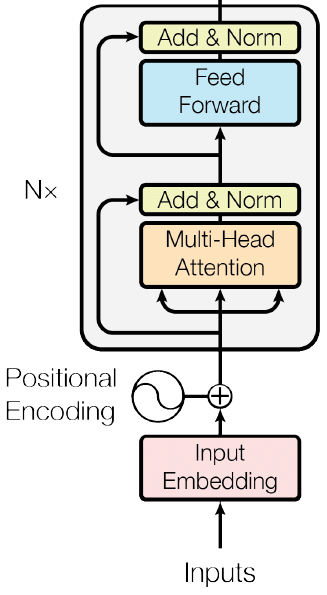
\includegraphics[width=0.25\textwidth]{Images/crossmodalnetworks/The-Transformer-encoder-structure.png}
        \caption{Image of a transformer used as a textencoder\cite{fig:encoder}.}
        \label{fig:crossmodalnetworks:textencoder}
    \end{figure}
    


    \section{Image encoder}
    The image encoder consists of a vision transformer\cite{Vis_N_Grams} in most cases.
    As the text encoder the vision encoder encodes a image in a high dimensional vector space.
    A vision transformer needs an image in a specific dimension.
    For that reason a Image encode is a pair of vision transformer and preprocessor which changes a imge to the right dimensions for the vision transformer

    
    \section{Contrastive Language-Image models
        \label{section:languageimagemodels}}
        In this section some models have been investigated which use contrastive language-image pretraining.
        Most of the information in this section are taken from \cite{cliplikeweb} and from the coresponding papers.

        Contrastive techniques take paired inputs from two modalities (e.g. an image and its caption).
        Both inputs are embedded in their own embedding space.
        The goal is for such a pair to be represented in a similar embedding by its corresponding encoder.
        Speech-image describes the two modalities used by a model.
        Pre-training means that the model has been trained on a large and universal dataset.
        These models are often refered to as foundational models.
        For a specific application, a pre-trained model can be fine-tuned to better perform its specific task.

        \subsection{CLIP
            \label{section:clip}}
        \acrfull{clip} \cite{clip} is a cross-modal model from openAI\cite{openai} which can tell how well a given image and a given text fit together.
        Its can be used with a variaty of image and text encoders.
        It is trained on a large Dataset, which consist of 400 million image-text pairs.
        On its realeas it outperformed some of the best known models.
        Many other model use CLIP as their base and build better models of it.

        \begin{figure}
            \centering
            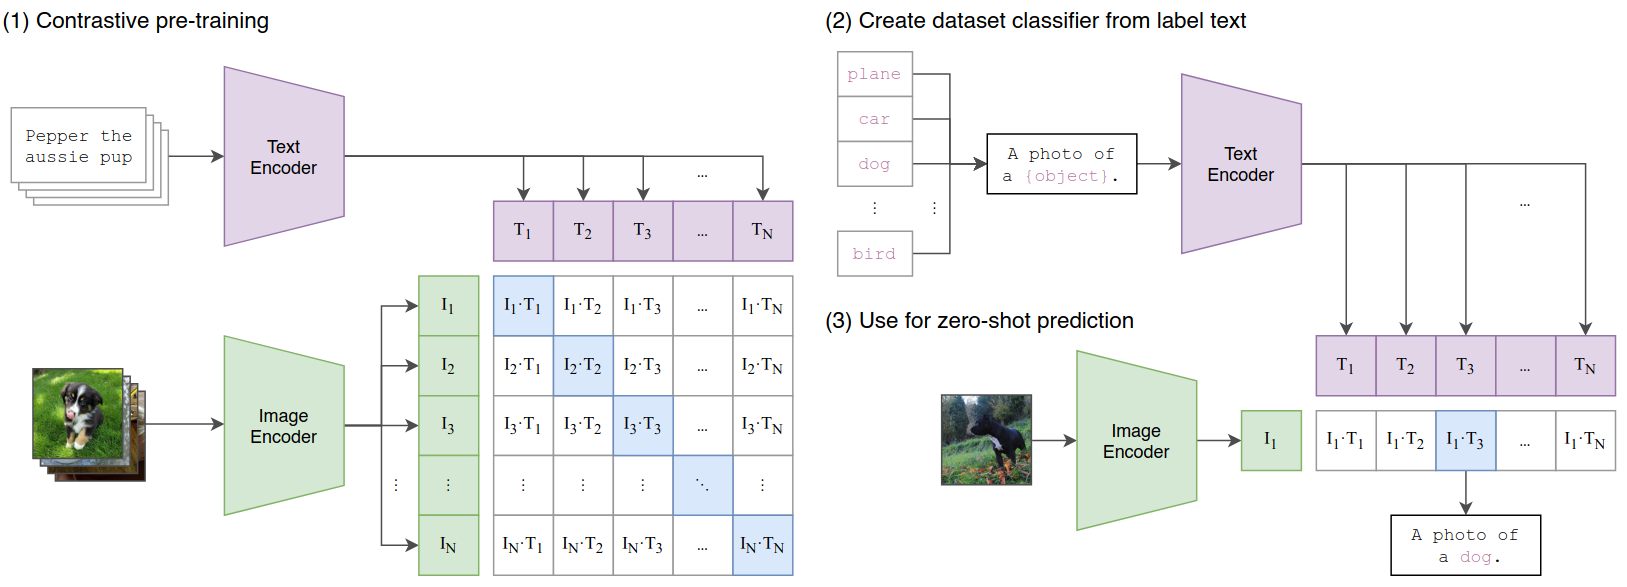
\includegraphics[width=\textwidth]{Images/crossmodalnetworks/OpenAICLIP.png}
            \caption{A picture from the \acrshort{clip} paper by OpenAI.}
            \label{fig:crossmodalnetworks:openaiclip}
        \end{figure}

        \subsection{ALIGN
            \label{section:align}}
        \acrfull{align}\cite{ALIGN} was published shortly after \acrshort{clip}.
        Rather than relying on small and image captioning dataset, \acrshort{align} uses dataset of \(1.8\) billion pairs of image and alt-text pairs(e.g. in \cref{fig:crossmodalnetworks:alignepairs}).
        These alt-text description are far more noisier than captions.
        The authors apply basic filtering to remove duplicates, images with more than 1000 associated alt-texts, and uninformative alt-texts (either too frequent or containing rare tokens), but avoid expensive filtering operations.
        With just these simple steps, ALIGN meets or exceeds the state of the art for several zero-shot and fine-tuning tasks.
        \begin{figure}
            \centering
            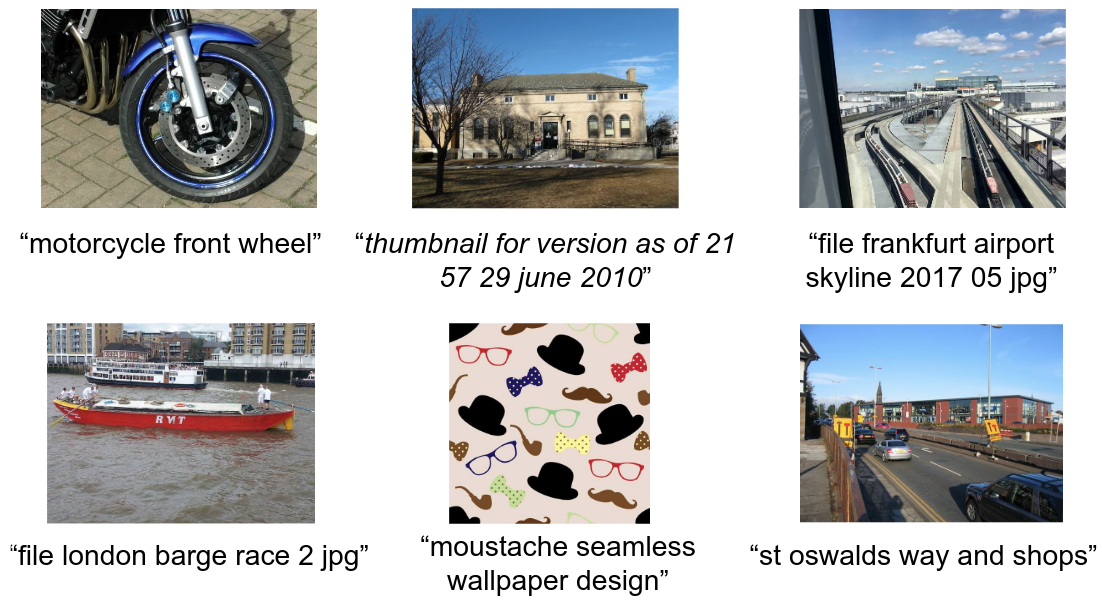
\includegraphics[width=\textwidth]{Images/crossmodalnetworks/examplepicsalign.png}
            \caption{Example of alt-text image pairs from the train dataset from \acrshort{align}}
            \label{fig:crossmodalnetworks:alignepairs}
        \end{figure}

        In a test for this work \acrshort{align} was much slower in computing a zeroshot evaluation on the CIFAR100\cite{cifar100} dataset than CLIP.
        For 1 prediction \acrshort{align} needs 70 times more time than \acrshort{clip} (see \cref{tab:clipaligntest}).
        Both networks are not finetuned. The highest predicted label is used. Due to the slow interferance ALIGN was stopped after it processed 35\% of the dataset.

        \begin{table}
            \centering
            \begin{tabular}{lll}
                \hline
            \textbf{Measurment}&\textbf{ALIGN}&\textbf{CLIP}\\\hline
            Accuracy& 48.9\% & 61.7\%\\
            Speed(seconds per iterarion)&  2.16&  0.02\\ \hline
            \end{tabular}
            \caption{First test on CIFAR100.}
            \label{tab:clipaligntest}
        \end{table}

        \subsection{TinyCLIP
            \label{section:tinyclip}}
        \begin{figure}
            \centering
            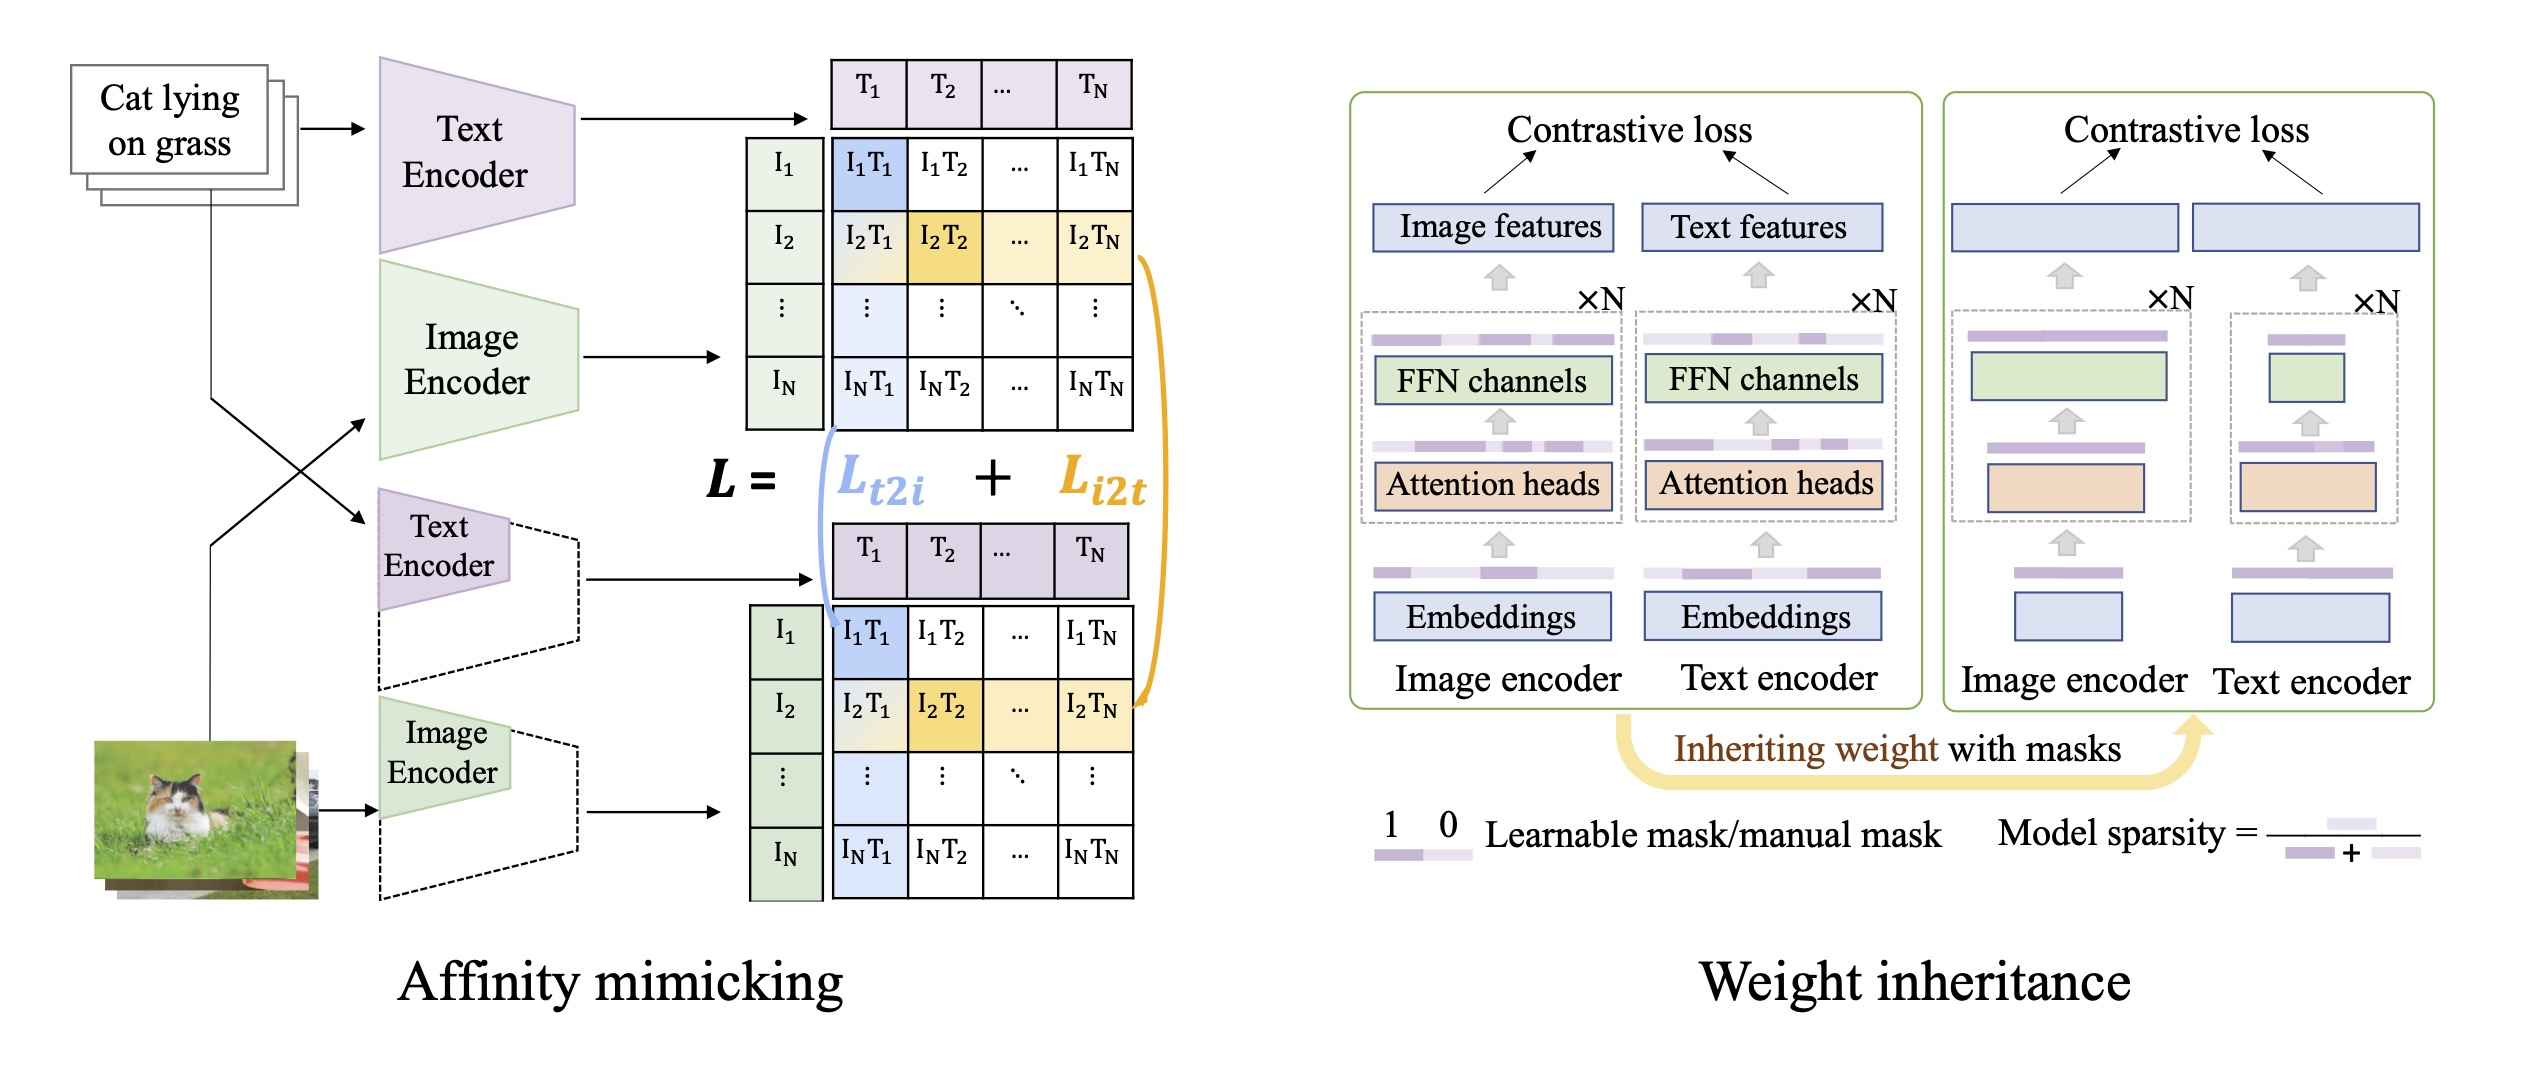
\includegraphics[width=\textwidth]{Images/crossmodalnetworks/TinyCLIP.jpg}
            \caption{Optimization which are used in TinyCLIP\cite{tinyclip}}
            \label{fig:crossmodalnetworks:tinyclip}
        \end{figure}

        TinyCLIP\cite{tinyclip} is a cross-modal distillation method for large-scale language-image pre-trained models.
        The miniaturisation makes it possible to use TinyClip on limited systems.
        It also speeds up interferance with a minimal loss of model accuracy.
        It uses 3 concepts to reduce the size of network.

        \subsubsection{Affiniy mimicking}
        Affiniy mimicking is a special form of knowledge distillation\cite{knowledgedistillation}, alsow called model distillation.
        In knowledge distillation, a larger teacher network is trained first.
        After training the teacher network, a smaller student network is trained to predict the output of the teacher network.
        This works because the output of the teacher network has more information than the original label.
        Affiniy mimicking uses two new metrics in training: language-to-image loss and image-to-language loss(\(L_{t2i}\) and \(L_{i2t}\) in \cref{fig:crossmodalnetworks:tinyclip}).

        \subsubsection{Weight inhertiance}
        Weight inheritance is a techinque which inherits the important weights from well-trained teacher models to smaller student models.
        In the paper the authors propose 2 methods:

        \subsubsection{Manual weight inhertiance}
        Based on observaitions of the authors.
        Text encoder have most redundancy in depth (layer-wise), image encoder in width (channel-wise).
        They select \(k\) layers and channels of a branch which will function as initialization weights.
        To select the most important weights prior knowledge is required

        \subsubsection{Automatic weight inhertiance}
        The Authors introduce a learnable mask to identify weight importance.

        \subsubsection{Multi-stage progressiv distillaiton}
        Pruning the model over multiple stages.
        For each stage the authors use a modest degree of compression (e.g. 25\%). Each stage includes weight inheritance and affinity mimicking.

        % Due to the fact that TinyCLIP is already available and is much smaller in comparison to the origibal it will be further used in this work.




    % \begin{table}
    %     \begin{tabular}{llll}
    %         \hline
    %     &  a Yahoo& ImageNet& SUN \\\hline
    %     Visual N-Grams&  72,4&  11,5&  23,0\\
    %     CLIP&  98,4&  76,2&58,5\\ \hline
    %     \end{tabular}
    %     \caption{Table 1. from \cite{clip}. Comparing CLIP to prior image zero-shot classification results\cite{Vis_N_Grams}}
    % \end{table}